\documentclass[11pt,letterpaper]{article}
% Add a bunch of useful math, font, and symbols
\usepackage{amsfonts}
\usepackage{amsmath}
\usepackage{amssymb}

% English support
\usepackage[english]{babel}

% Background image support
\usepackage[pages=some]{background}

\usepackage{booktabs}

% Citation
\usepackage[superscript]{cite}

% Better enumerate and itemize
\usepackage{enumitem}

% Better control of headers and footers
\usepackage{fancyhdr}

% Floating objects like figures and tables
\usepackage{float}

% Page layout and dimensioning
\usepackage[margin=1in]{geometry}

% Basic color, graphics and text manipulation 
\usepackage{graphicx}

% Use Helvetica typeface
\usepackage[scaled]{helvet}
\renewcommand\familydefault{\sfdefault} 
\usepackage[T1]{fontenc}

% Cross-referencing hyperlinks
\usepackage{hyperref}

% Line break for long URLs
\usepackage{breakurl}

% Accept utf-8 input encoding
\usepackage[utf8]{inputenc}

% Make indexes
\usepackage{makeidx}

% Microtype (apparently makes the typographics stuff better)
\usepackage{microtype}

% multi-column writing
\usepackage{multicol}

% English ordinal counting (1st, 2nd, etc.)
\usepackage{nth}

% Long table
\usepackage{longtable}

% Paragraph skip - adds extra lineskip spacing
\usepackage{parskip}
\setlength{\parskip}{0.7\baselineskip plus 2pt}

% Add ability to set space between lines
\usepackage{setspace}

% S.I. units
\usepackage{siunitx}

% Subcaptions for subfigures
\usepackage{subcaption}

% Include svg graphics
\usepackage{svg}

% Drawing graphics
\usepackage{tikz}

% Subsubsubsection
\usepackage{titlesec}
\setcounter{secnumdepth}{4}
\titleformat{\paragraph}
{\normalfont\normalsize\bfseries}{\theparagraph}{1em}{}
\titlespacing*{\paragraph}
{0pt}{3.25ex plus 1ex minus .2ex}{1.5ex plus .2ex}

% Custom titles
\usepackage{titling}

% Url
\usepackage{url}

% Figure frame
\usepackage{mdframed}

% Listing
\usepackage{listings}

\RequirePackage[figure,table]{totalcount}


% Custom definitions
\newcommand{\doctitle}{P3C: Technical Report}
\newcommand{\docsubtitle}{Are You Looking at Me? Eye Gazing in Web Video Conferences}

% Custom commands
\newcommand{\ts}{\textsubscript}	% Subscript command %
\newcommand{\revisionnum}{!! Revision number not found. Please add renew command \\revisionnum in the document after the ``aliases.tex'' include !!}
\renewcommand{\revisionnum}{1.3}
% Use hyphans to break up urls
\def\UrlBreaks{\do\/\do-}

% PDF and href setup
% Hyper ref
\hypersetup{
	colorlinks=true,
	citecolor=black,
	linkcolor=black,
	filecolor=black,
	urlcolor=blue,
	pdftitle={\@title},
	bookmarks=true
}
\urlstyle{same}
% Page headings
\pagestyle{fancy}
\fancyhead[L]{\MakeUppercase{CPEN 541}}
\fancyhead[C]{\textbf{\doctitle}}
\fancyhead[R]{Group 8}
\fancyfoot{}
\fancyfoot[C]{}
\fancyfoot[R]{\thepage}

% No paragraph indent
\parindent 0ex

% Meta
\author{
	He, Muchen &
	\texttt{44638154} &
	\textit{mhe@ece.ubc.ca}
	\\
	Xia, Kaseya &
	\texttt{27553304} &
	\textit{zxia@uvm.edu}
	\\
	Xiong, Beibei &
	\texttt{13233747} &
	\textit{beibei971030@gmail.com}
}
\title{\doctitle}
\date{\today}
\makeatletter
\renewcommand{\maketitle}{
	\bgroup
	\setlength{\parindent}{0pt}
	\begin{flushleft}
		% Top spacing
		\vspace*{0.5in}

		% Team logo
		
\includegraphics[scale=0.158]{../assets/logo.png}
		\vspace*{0.25in}

		% Title
		\textbf{\Huge{\@title}}\\
		\hrulefill

		% Subtitle
		\textbf{\huge{\docsubtitle}}
		
		\vspace*{0.5in}

		% Course number and team
		\textsc{\scriptsize{\textbf{STUDENT GROUP}}}\\
		\textbf{\Large{Group 8}}\\
		\hspace*{0.1cm}
		\begin{tabular}[h]{|ll}
			\@author
		\end{tabular}

		\vspace*{0.25in}

		\textsc{\scriptsize{\textbf{INSTRUCTOR}}}\\
		{\textbf{\Large{Dr. Sidney Fels}}}\\
		\hspace*{0.1cm}
		\begin{tabular}[h]{|ll}
			Electrical and Computer Engineering, The University of British Columbia
		\end{tabular}

		\vfill
		
		% Date
		\large{Revision \revisionnum~---~\@date}
		\vspace*{0.5in}

		% Logo
		\hspace*{-0.3cm}
\includegraphics[scale=0.5]{../assets/ece_logo.pdf}

	\end{flushleft}
	\egroup
}
\makeatother

% Begin Document
\begin{document}
% Title Page
\begin{titlepage}
	\maketitle
\end{titlepage}


\renewcommand{\thepage}{\roman{page}}
\setcounter{page}{1}

% Revision history
\backgroundsetup{
	scale=1,
	color=black,
	opacity=0.3,
	angle=0,
	contents={\includegraphics[height=\paperheight,width=\paperwidth]{../assets/render2bg}}
}
\BgThispage
%\thispagestyle{empty}
\section*{Revision History}
The full revision history and commited changes of the document can be found in the git repository history: \href{https://github.com/Capstone-Skynet/Capstone-Skynet.github.io}{https://github.com/Capstone-Skynet/Capstone-Skynet.github.io/commits/master}.

\begin{table}[H]
\begin{tabular}{*{4}{l}p{0.5\linewidth}}
\hline
Version \# & Initials & Release Date & Changeset & Changes Made \\ \hline

0.0 & PD & 2019-10-11 & \texttt{660e001} & Initial skeleton of the document.\\
0.1 & MH & 2019-10-11 & \texttt{6af9e8a} & Populate initial document with draft content required for Milestone I.\\
1.0 & PD & 2019-11-23 & \texttt{} & Updated header to synchronize styles for Milestone II.\\
1.1 & PD & 2020-04-06 & \texttt{} & Updated physical computation platform deliverables.\\
1.2 & PD & 2020-04-08 & \texttt{} & Updated delivery instructions.\\
1.3 & MH & 2020-04-08 & \texttt{b1680955} & Final revision for M4.\\
 & & & \\ \hline
\end{tabular}
\end{table}

\clearpage

% Table of contents
\setcounter{secnumdepth}{3}
\tableofcontents
\thispagestyle{empty}

% Roman numeral page numbers


% Terms and Abbreviations
\section*{Terms and Abbreviations}
\addcontentsline{toc}{section}{Terms and Abbreviations}

\textit{No new terms are utilized in this document.}


% List of figures and tables
\iftotalfigures
\addcontentsline{toc}{section}{\listfigurename}
\listoffigures
\fi
\iftotaltables
\addcontentsline{toc}{section}{\listtablename}
\listoftables
\fi

\newpage

% Set page and section counter
\renewcommand{\thepage}{\arabic{page}}
\setcounter{page}{1}

\section*{Preface}

This document is intended for the instructor or students of the human-computer interface course CPEN 541 to learn and possibly reproduce the experimental setup and results. The document outlines in detail the research questions we are pursing, as well as the motivation. This document also describe the prototype and its experiments we developed to test our research questions along with our findings. Lastly, this document features the limitations as well as the future work (including what the prototype would ideally look like). 

Please also refer to our other submitted work, including our conference paper, demonstrative video, and presentation slides.

We can be contacted via our emails (listed at the top of the document). All the code for this project can be found on GitHub: \url{https://github.com/CPEN541-FutureGazer}.

\clearpage

\section{Introduction and Problem}

Over the last year, we all observed and experienced first-hand at attempting to scavenge the productivity and work-ethics we once had while working from home while in a pandemic. And one of the most important work-related ritual is none other than meetings and hangouts. 

As limited by the restriction and the isolation to curb the infectious virus, we sacrificed the ability to meet with people face-to-face (F2F) --- whether that be getting work done, attending classes, discussing and brainstorming ideas, and even asking for help and or assistance from peers. Out of necessity, we all forced to use online web-video-conferencing (WVC) software such as Zoom, Skype, etc. as a substitute.

Despite these companies touting the technological advancements, the intuitive of its user-interfaces, the affordable cost of “free” to its users, they all had this one *glaring* (pun-intended) problem that none of these software truly provided in the absence of F2F meetings: that \textbf{eye-contact} and \textbf{gaze} are an essential part of body language and non-verbal communications in social situations. 

Conventional WVC software evolved from 1-on-1 meetings, where the only other person on the screen is the one you talk to, like in a phone call. This has the few problems of modern, large meetings involving more people, since the other person’s face is the only thing you look at and thus easier to make eye-contact and attention. 

\begin{figure}[H]
	\centering
	% \includegraphics[width=0.85\textwidth]{img/multirotor.png}
	\caption{Quadcopter X-Configuration}
	\label{fig:test1}
\end{figure}

However, seen in the image below, as we add more participants to the meeting, instead of being an intimate experience, we are often presented with a gallery, somewhat like a bookshelf view of all the participants. Each participant is placed in a uniform cell as part of a grid. One could describe it as a jail-cell, lacking in connection, organicity, and coherency. Furthermore, because everyone is looking at their own screen, towards their camera, we get a mostly static view of all the participants looking out of the screen on the receiving end. Somewhat akin to have a large audience all staring at you --- even if you’re one among them passively listening.

`insert gallery view of zoom` in contrast with `image of people sitting around a table looking at each other`

\section{Background and Prior Works}

A large body of prior work has explored that eye contact is a critical aspect of human communication. [1, 2] Eye contact plays an important role in both in person and a WVC system. [3, 4] Therefore, it’s critical and necessary to preserve eye contact in order to realistically imitate real-world communication in WVC systems. However, perceiving eye contact is difficult in existing video-conferencing systems and hence limits their effectiveness. [2] The lay-out of the camera and monitor severely restricted the support of mutual gaze. Using current WVC systems, users tend to look at the face of the person talking which is rendered in a window within the display(monitor). But the camera is typically located at the top of the screen. Thus, it’s impossible to make eye contact. People who use consumer WVC systems, such as Zoom, Skype, experience this problem frequently. This problem has been around since the dawn of video conferencing in 1969 [5] and has not yet been convincingly addressed for consumer-level systems.

Some researchers aim to solve this by using custom-made hardware setups that change the position of the camera using a system of mirrors [6,7]. These setups are usually too expensive for a consumer-level system. Software algorithms solutions have also been explored by synthesizing an image from a novel viewpoint different from that of the real camera. This method normally proceeds in two stages, first they reconstruct the geometry of the scene and in second stage, they render the geometry from the novel viewpoint. [8, 9, 10, 11, 12] Those methods usually require a number of cameras and not very practical and affordable for consumer-level. Besides, those methods also have a convoluted setup and are difficult to achieve in real-time.

Some gaze correction systems are also proposed, targeting at a peer- to-peer video conferencing model that runs in real-time on average consumer hardware and requires only one hybrid depth/color sensor such as the Kinect. [13] However, when there are more than two persons involved in a web video conference, even with gaze corrected view, users still cannot tell whether a person is looking at him or someone else in the meeting. With the gaze correction, it will create the illusion that everyone in this meeting is looking out of the screen. This could cause a serious confusion.


\subsection{Eye Contact in Multi-person Conversation}

Most studies of eye contact during conversations focused on two-person communication [14]. 
However, multi-person conversational structure becomes more complicated when a third speaker is introduced. It has long been presumed that eye contact provides critical information in conversations. Isaacs and Tang [15] performed a usability study of a group of five participants using a desktop video conferencing system. They found that during video conferencing, users addressed each other by name and started explicitly requesting individuals to start talking. In face-to-face interaction, they found people used their eye gaze to indicate whom they were addressing. Sellen [16] was one of the first to formally investigate the effects of eye contact on the turn taking process in four-person video conferencing. Unfortunately, she found no effects because the video conferencing system she implemented did not accurately convey eye contact [16]. Vertegaal et al. [17] found that without eye contact, 88\% of the participants indicated they had trouble perceiving whom their partners were talking to.

Therefore, we propose our system

NOTE: ALL References can be found in Latex


`insert existing solution`

`insert VR 3d chat apps`

`insert other research work`

\section{Research Questions and Scope}

This motivated us to explore alternative ways to represent participants in WVC applications to increase engagement, interactivity, and attention. 

In distant-learning classes, for example, presenters (e.g. professors, teachers, students) often feel distracted or disengaged when there are no audiovisual feedback coming from the audience. These feedback include eye contact, gaze direction, and other body language cues.

We are set out to build a prototype WVC application to study the perceived effects of eye-contact, gaze, and head orientation in a virtual 3D space to make up the missing aspects from in-person F2F interactions.

Our project explores whether adding eye-contact to the current WVC system will enhance the sense of interaction and presence of the users. Conventional WVC services only offer standard visual and audio communication, and they do not support intuitive and personalized eye-contact between users. Therefore, people still prefer face-to-face meetings because of the highly interactive meeting environment.

We propose FutureGazer, a WVC system that simulates eye-contact and gaze amongst the participants in a WVC meeting room to enable a highly interactive environment. Our project explores whether adding eye-contact to the current WVC system will enhance the sense of interaction and presence of the users. Conventional WVC services only offer standard visual and audio communication, and they do not support intuitive and personalized eye-contact between users. Therefore, people still prefer face-to-face meetings because of the highly interactive meeting environment\cite{rn42}.

To test our system, we recruit friends and students are participants to study the effects of the additional eye contact and gaze cues in online meeting environments. Figure \ref{fig:intro-a} shows what we intend to build in contrast to existing WVC platforms like Zoom. Figure \ref{fig:intro-b} depicts the personalized eye-contact simulation enabled by our system.

\begin{figure}
	\centering
 	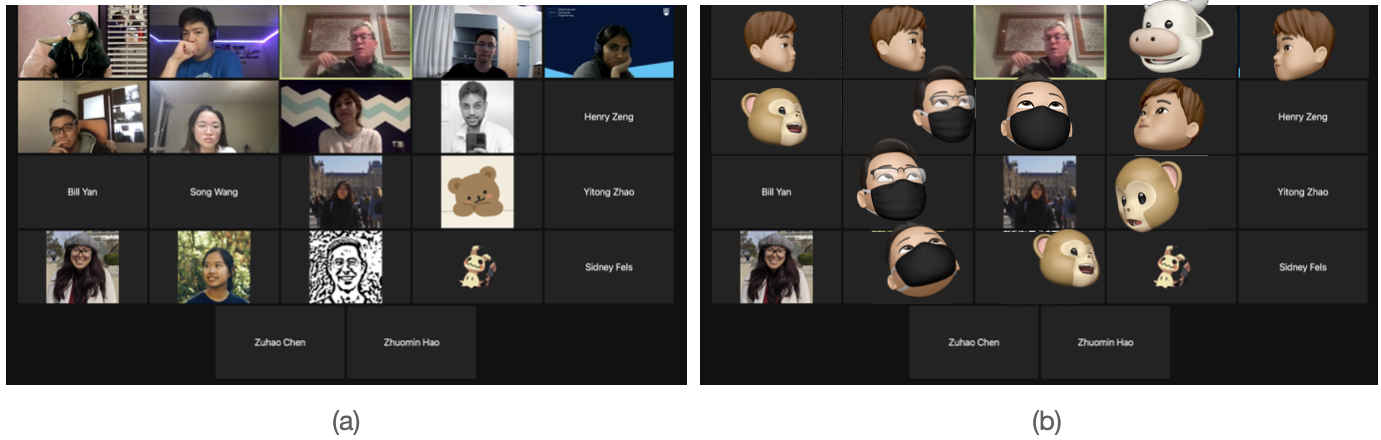
\includegraphics[width=0.9\textwidth]{introA.png}
	\caption{(a) Current WVC model: each participant stays in their grid and no eye contact interaction. (b) Proposed model: students can look at each other to create virtual eye-contact.}
	\label{fig:intro-a}
\end{figure}

\begin{figure}
	\centering
 	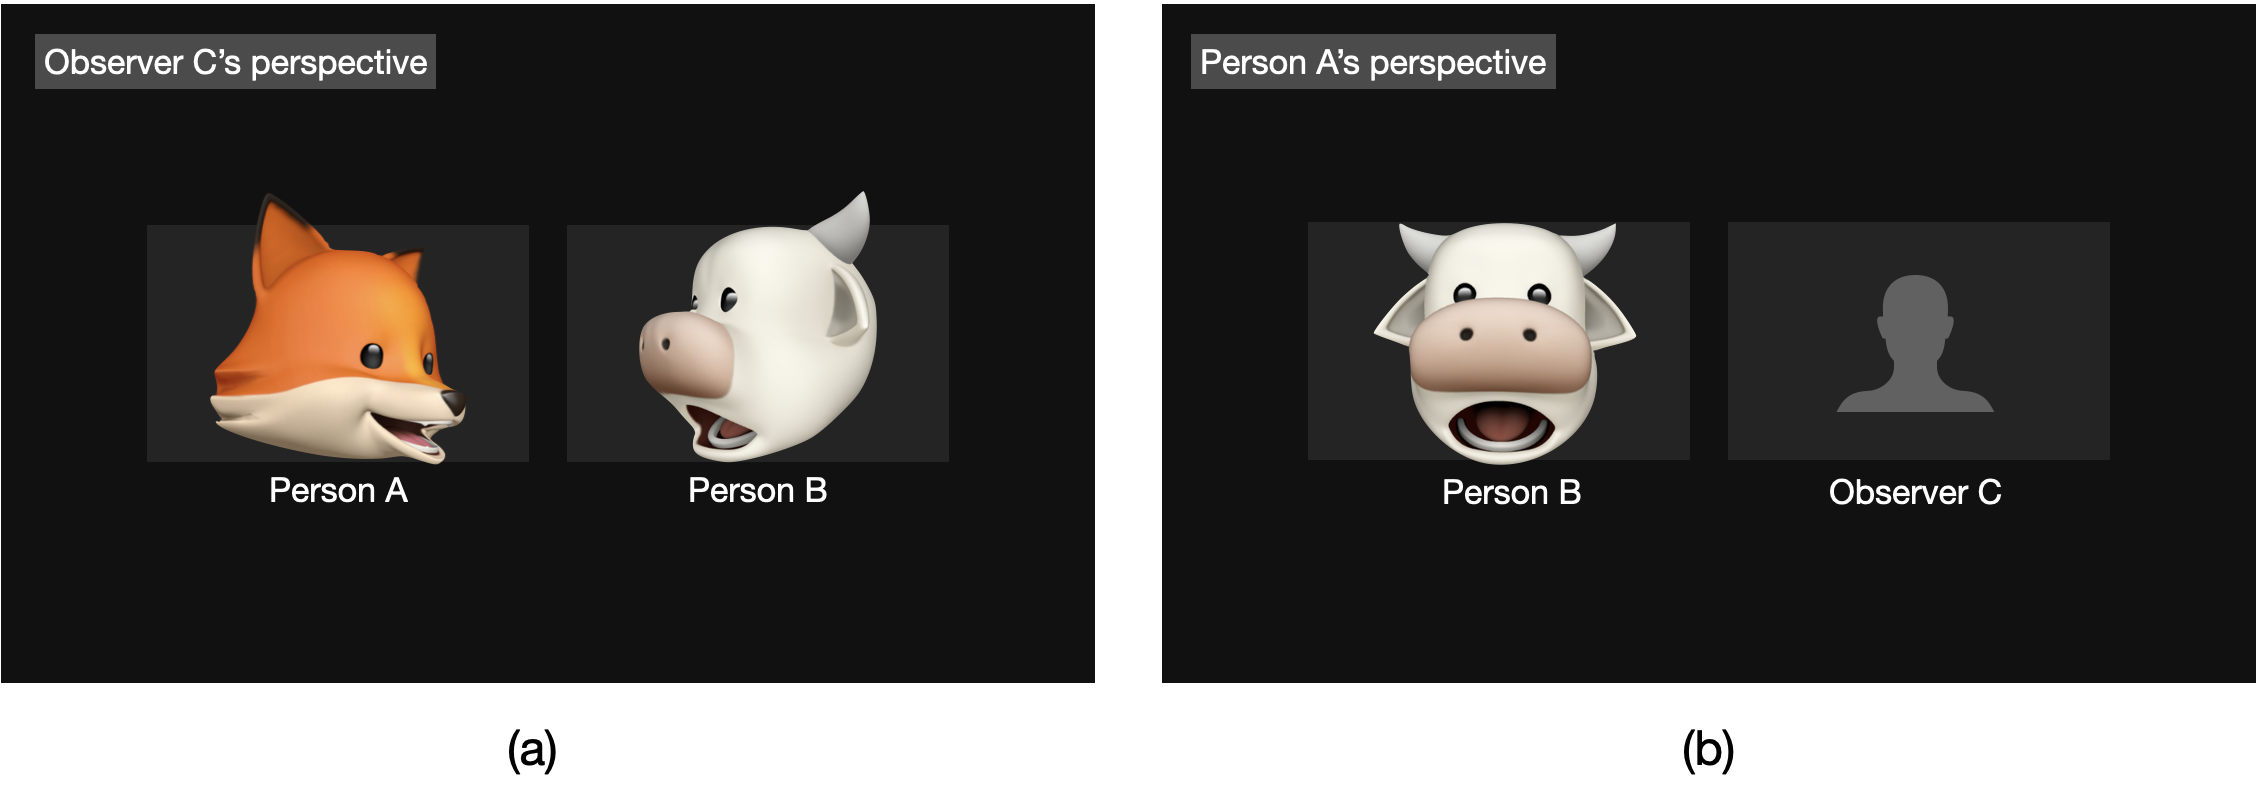
\includegraphics[width=0.9\textwidth]{introB.png}
	\caption{(a) Observer’s perspective in a meeting room with person A (fox) and person B (cow) looking at each other. (b) Person A’s perspective in the exact same meeting room at the exact same time.}
	\label{fig:intro-b}
\end{figure}

The key metrics we want to observe in this project are: participant’s attention, engagement, and the feeling of connectedness. To explore parameters that effect these metrics, we consolidate these ideas into three core research questions (hereafter will be refer to as \textbf{RQ1}, \textbf{RQ2}, and \textbf{RQ3}):

\begin{enumerate}
    \item Can a person tell if they are being looked at in a WVC and how can 3D avatars be augmented to enhance this experience.
    \item Can a person tell if other participants are looking at each other in a WVC and how using 3D avatars can be augmented to increase engagement.
    \item How does a person’s attention change as the avatars augmented with WVC enables eye-contact and gaze.
\end{enumerate}


\section{The Prototype}

This section describes the technical details regards to our implementation. We first outline the language and framework this prototype is developed on, then we describe the rendering, layout, and orientation calculation. Lastly we go over the configuration files, events, timed and randomized sequences, and integrated questionaries that aid us in user-experimentation.

Note: Since this project is not mainly focused on the usability study of this concept, we only implemented the minimum-viable-product to carry-out the user experiments due to time-constraints. We discuss how this prototype could be improved in future>prototype section.

\subsection{Platform}

The prototype is mostly developed in Processing cite (a Java-based graphic-centric language mostly used in education, prototype, and visual arts) and Unity Engine cite (a popular free-to-use game engine). The Unity engine wraps around the Processing prototype to provide user-testing interface such as integrated questionaries and videos.

We chose Processing and Unity as they have strong support of 3D environment, video and audio playback, robust mouse input, ease-of-use, and quick prototype turn-around overheads. Both frameworks are also cross-platform and can execute on Windows, macOS, and Linux. However, as we also discuss in Section limitations section, recent macOS cite macOS update added a *Gatekeeper* security feature that prevents un-sighed software from running --- thus complicating the user-testing process, as distributed prototype executables to the participants cannot be opened.

\subsection{3D Environment}

insert figure of a typical view of the prototype in Unity app

Figure insert figure shows a typical 3D environment rendered in the prototype app. We base the user interface (UI) design --- including colours, buttons, and layout --- from existing WVC apps such as Zoom to present the participants with a familiar user experience. By doing so, we limit other factors that would interfere with our user experiments. However unlike traditional WVC apps, we replace the centre (where typically there would be a gallery or grid view of camera video feeds) with our prototype avatar representation.

From hereafter, we will refer to these visual representation of participants in the meeting as *Avatar Views* (*View* class). As outlined earlier in [Section on research questions](research-questions-and-scope), we propose two types of avatars to explore: 3D head avatars (*HeadView* class) and 2D eye avatars (*EyeView* class). 

insert figure of head view class and the eye view class

For user experiments, we create *mock avatars* to replicate/simulate real meeting participants. This creates an illusion for the test participants as if they’re real people to help us speed up the testing process without involving lots of people. However, as it is an illusion, it might affect how people perceive our prototype --- as we discuss in [Section 7. Limitations](limitations). 


\subsubsection{Heads}

show image of 3d model of the head

insert head avatar grid view

In the 3D environment, the head avatars are loaded from a free-to-use .OBJ 3D model downloaded from *TurboSquid* with standard usage license cite 
%[^:https://blog.turbosquid.com/turbosquid-3d-model-license/Educational-Use]. 
We load the object into the 3D scene once, and use the same model instance for all other head avatar *HeadView* objects to save computation --- since they’re essentially the same 3D model, just redrawn with different transformations.

Due to time and budget constraints, we are limited to a low-polygon-count model of the head, with no texture, no rigging, no soft-body animation, and no physics simulation. The 3D model of the head, as shown in Figure TODO, has minimum features of a face. Despite the low-quality 3D models, the primitiveness of the 3D model helps maintaining a high rendering frame-rate while the prototype is running, even without writing custom shaders and performing fine-tuned optimizations --- especially when there could potentially be up to 9 to 25 avatars being drawn concurrently on to the screen. This is important as we need the head avatars to transform and render in real-time as if they’re real inputs in a WVC application.
As we will discuss in Section TODO: future work, if given more budget and 3D talent, more work can be allocated to polishing the visual appeal of the avatars to be more inviting and friendly, and ultimately improve user-experience.

\subsubsection{Eyes}

The 2D eyes avatar was inspired from goggly eyes and novel desktop widgets (e.g. XEyes TODO: cite) created as general amusement. However, we decided to explore this as an alternative to the head avatars to see whether if 3D and head orientation is required to deliver eye-contact and gaze hints to the meeting participants. 

insert breakdown diagram of the eye rendering

insert eye avatar view

insert eye avatar grid view

With eyes avatars, instead of a 3D object transformed to orient a direction, we simply render a pair of pupils and irises on a white background as a sub-image (Figure TODO). Then depending on where the eye should be looking at, we rendering this sub-image with a transform that translates it in $x$ or $y$ direction (Figure TODO). Finally, we create an eye mask that only only renders the eye itself (Figure TODO).

The result is somewhat similar to a gallery view of meeting participants in a traditional WVC application, except with only the eyes and their gaze visually represented.

\subsubsection{UI Elements}

As discussed in Section TODO (3d-environments) seen in Figure TODO (from 3d-environment section). The 3D head avatars and 2D eye avatars are rendered at $z=0$. In front of that, we render the UI elements such as the bottom menu bar, as well nameplates to aid in our experiments and to provide a familiar environment to the participants.

insert image of talking halo

When a participant corresponding to an avatar is talking, we have an option to activate a yellow halo behind the avatar for indication. To do this, each avatar *View* base class has a flag isFocused that can be toggled. If this flag is on, then we draw this additional halo on a layer behind the avatars.

insert image of the point light source

While not used in our final experiments, we also added an option to highlight avatars in on the screen based on mouse cursor positions. Rather than drawing a bounding box around the avatar, we thought it was appropriate to instead model the mouse cursor effects as a point-source-light with some vibrant colour, such as seen in Figure TODO. This option can be turned on via experiment configuration file (see Section TODO: configuration file). 

\subsection{View Modes}

To simplify the behaviour of mock avatars, we have three pre-programmed modes for the avatars to follow:

\begin{enumerate}
    \item \textbf{NORMAL}: the avatar is in normal mode, it will follow and track a given set of target coordinates (see [Section TODO](target-coordinates)).
    \item \textbf{STARE}: the avatar should stare at the active participant by gazing directly outwards from the screen.
    \item \textbf{RANDOM}: the avatar randomly looks around as if they are distracted. Current implementation of the random mode uses a series of Perlin noise functions to approximate how real head moves around randomly.
\end{enumerate}

Note that this would only apply to the mock avatars used in user experiments to simulate real people.

During user experiments, we can dynamically and programmatically change the modes of the avatars to simulate whether a person in the meeting is paying attention or not paying attention, and looking at the test subject participant, or anywhere else on the screen.


\subsection{View Calculation}

This section talks about the math and algorithms created to compute the target coordinates --- the screen-space coordinates of where that avatar should be looking at. As well as the mapping between the target coordinates to a rotation (for head avatars) or a translation (for eye avatars) transformations.

\subsubsection{Target Coordinates}

Each avatar (*View* base class) has attributes targetX and targetY which corresponds to where the avatar should directly look at in *normal* mode. These attributes are not used in *random* and *stare* modes.

For example, if the avatar is set to track the mouse cursor’s screen position, then we trivially set:

\begin{lstlisting}[language=Java]
avatar.targetX = mouseX
avatar.targetY = mouseY
\end{lstlisting}


If an avatar A is set to look at another avatar B, we can set the target coordinates of A to the spatial coordinates of B:

\begin{lstlisting}[language=Java]
A.targetX = B.x
A.targetY = B.y
\end{lstlisting}

\subsubsection{Rotation Calculation}

Once an avatar knows \textit{where} to look (i.e. the target coordinates),
it needs to compute \textit{how} to look in that direction (i.e. compute the corresponding transforms required to show the correct visual representation).

insert image of mapping from targetXy to offset Xy

For the 2D eye avatars, this mapping from target coordinates to transformation is a simple 2D translation $(\Delta x, \Delta y)$, as seen in Figure TODO. First, a difference vector $\vec d$ is computed from the avatar’s local origin to the target coordinates. We then scale it by some factor $s$ to control the sensitivity of this translation. Finally, we constrain the magnitude of $s\vec d$ to the radius of the eyes to ensure the pupil do not go off the eye, creating a white eye.

For the 3D head avatars, the mapping is instead from the target coordinates to a set of rotations along the x, y, and z-axis. The simplest way to do this is to draw a 3D vector from the head avatar origin to the target coordinates. Then using trigonometry on the vector, we can find all angles corresponds to the x, y, and z rotations.

Notice, that up to this point, we have not established the third, z-component, of the target coordinates. This is because it depends on what the head avatar should be looking at. If the avatar is looking at another avatar, we leave $z = 0$ since all avatars are on the $z = 0$ plane. However, if the avatar were to follow the mouse or stare at the user, then we must set $z = z^\prime$, where $z^\prime$ is the z-offset of the camera. The difference between with vs. Without this z-correction can be seen in Figure TODO

insert figure of heads looking straight on vs at the camera

\subsubsection{Realism Approximations}

For both eye and head avatars, instead of applying the transformation in the renders according to he target coordinates instantaneously, we use a linear-interpolation function to smoothen the motion and simulate a more natural response --- a response with mass, inertia, and a sense of reaction time delay that would exist in real people.

We also added an option to make the head wobble controlled by some noise to make the avatars feel less robotic and more organic. If a 3D head avatar’s isFocused flag is set on (such as when the participant the avatar belongs to is speaking), the wobble amplitude is slightly increased to approximate the extra motion due to mouth movements.

\subsection{Configuration Files}

To facilitate a series of automated, consistent, yet randomly generated user experiment scenarios, we developed a configuration framework for our prototype. Each experiment setup (see [Section TODO](experiment-setup)) is contained inside a config.json file. Each file contains all the experiment parameters such as number of avatars, type of avatars, names, and the sequence of modes, target coordinates, etc. 

\subsubsection{Initialization}

The file can be loaded at initialization-time of the experiment. Upon which, all the parameters in the configuration file is read, and the defined avatars are populated in the scene. 

\subsubsection{Events}

The sequence of state changes in the prototype user experiment is controlled by *events*. These events are defined in the configuration files as a single array that represents a timeline. The different types of events supported are:

\begin{itemize}
    \item Change mode
    \item Change avatar target
    \item Set focus flags
    \item Play sound
    \item Stop experiment
\end{itemize}

For more details regarding events, please refer to the source code.

\subsection{Unity Engine Wrapper}

To further facilitate user testing, we wrapped the Processing prototype in a Unity engine user interface, where participants are guided without the constant supervision from us. Each experiment setup is sequenced in order and appropriate questionaries are prompted in between each setup. Finally, the questionnaire responses are automatically logged in participants’ computer, making it easy for review.

\section{Experiment Setup}

- Recall research questions
- In pursuit of these answering these questions, we proposed these experiments that study how users feel about interacting using our prototype
- Describe all the different experiment configurations

\section{Evaluation \& Results}

\begin{figure}
	\centering
 	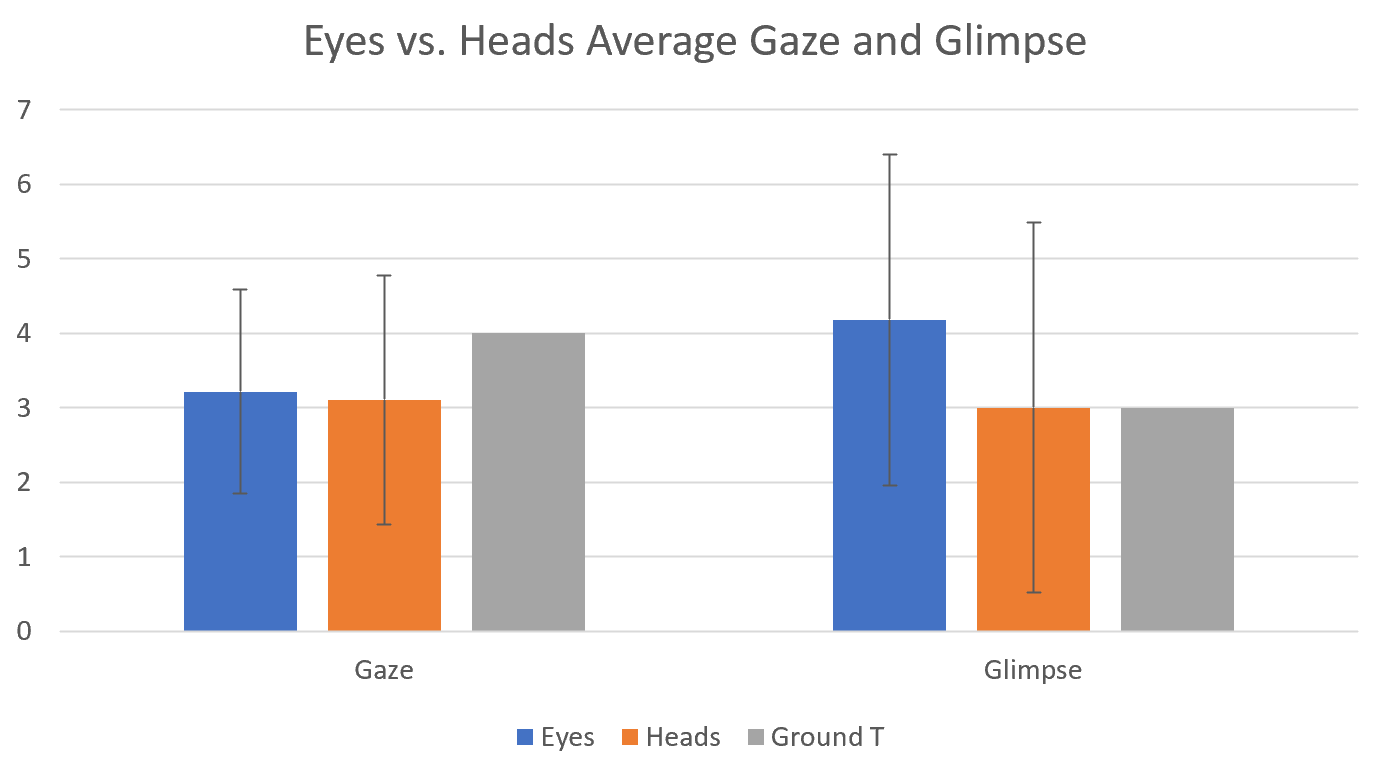
\includegraphics[width=\textwidth]{Result_F1.png}
	\caption{The eye model and head model gaze and glimpse times comparison with ground truth}
	\label{fig:e1-ga}
\end{figure}

In E1 experiment, all participants reported that they had been looked at. But in experiment H2, 14/15 participants reported that they had been looked at. The Figure \ref{fig:e1-ga} shows the gaze and glimpse number in both experiments E1 and H2 . The glimpse result is more sparse with the highest reported number being 9 (For E1), and the lowest being 1.5. This result matches our expectation. 

We did not reveal the questions before the experiments because we think it will cause the participants to pay extra attention to finding the answers, which will corrupt the original experiment purposes. Instead we only asked the participants to observe carefully while performing the experiments. Thus it’s expected that participants could not remember exactly what they just saw when answering those questions. We believe this created some outliers. For example, P11 is the only one who reported he had not been looked at in the H2.

We asked the participants ``Which one attracted your attention more: eyes(0) or heads(100)?" three times during the experiments. ``Watching" is E1 and H2, ``speaking" is after E3 and H3, and ``overall" is in the final question section. Results show that with all the tasks, participants felt their attention was attracted by the head model more than the eye model. Both the eye model and the head model universally make participants notice that they were being looked at. Participants have a sense of being looked with an average of 70.86\% due to the head and 29.14\% due to eyes (i.e. 3D heads make it more obvious to feel the glimpse and gaze), shown in Figure \ref{fig:e1-eye-vs-head}. 

\begin{figure}
	\centering
 	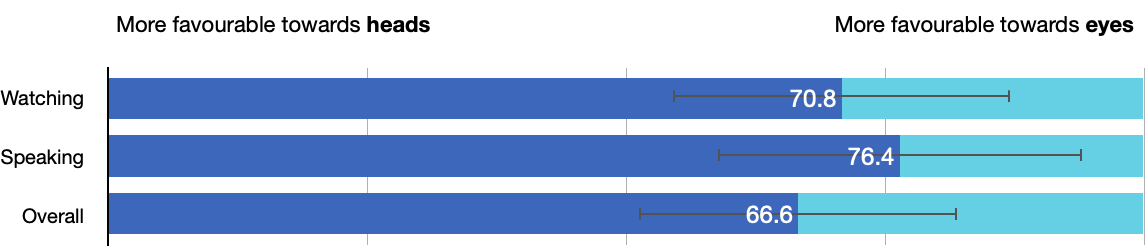
\includegraphics[width=\textwidth]{Result_F4.png}
	\caption{The attention distribution of heads and eyes in watching, speaking and overall tasks}
	\label{fig:e1-eye-vs-head}
\end{figure}

In experiment E3 and experiment H3, participants were asked to rate their nervous level, focus level, and engagement level compared with traditional WVC when using the eye model and the head model. As shown in Figure \ref{fig:e3h3}, 0 indicates our model is 100\% less nervous, focusing and engaging than the traditional WVC. 100 indicates our model is 100\% more nervous, focusing, and engaging than traditional WVC. 50 indicates our model is equivalent with traditional WVC. 

\begin{figure}
	\centering
 	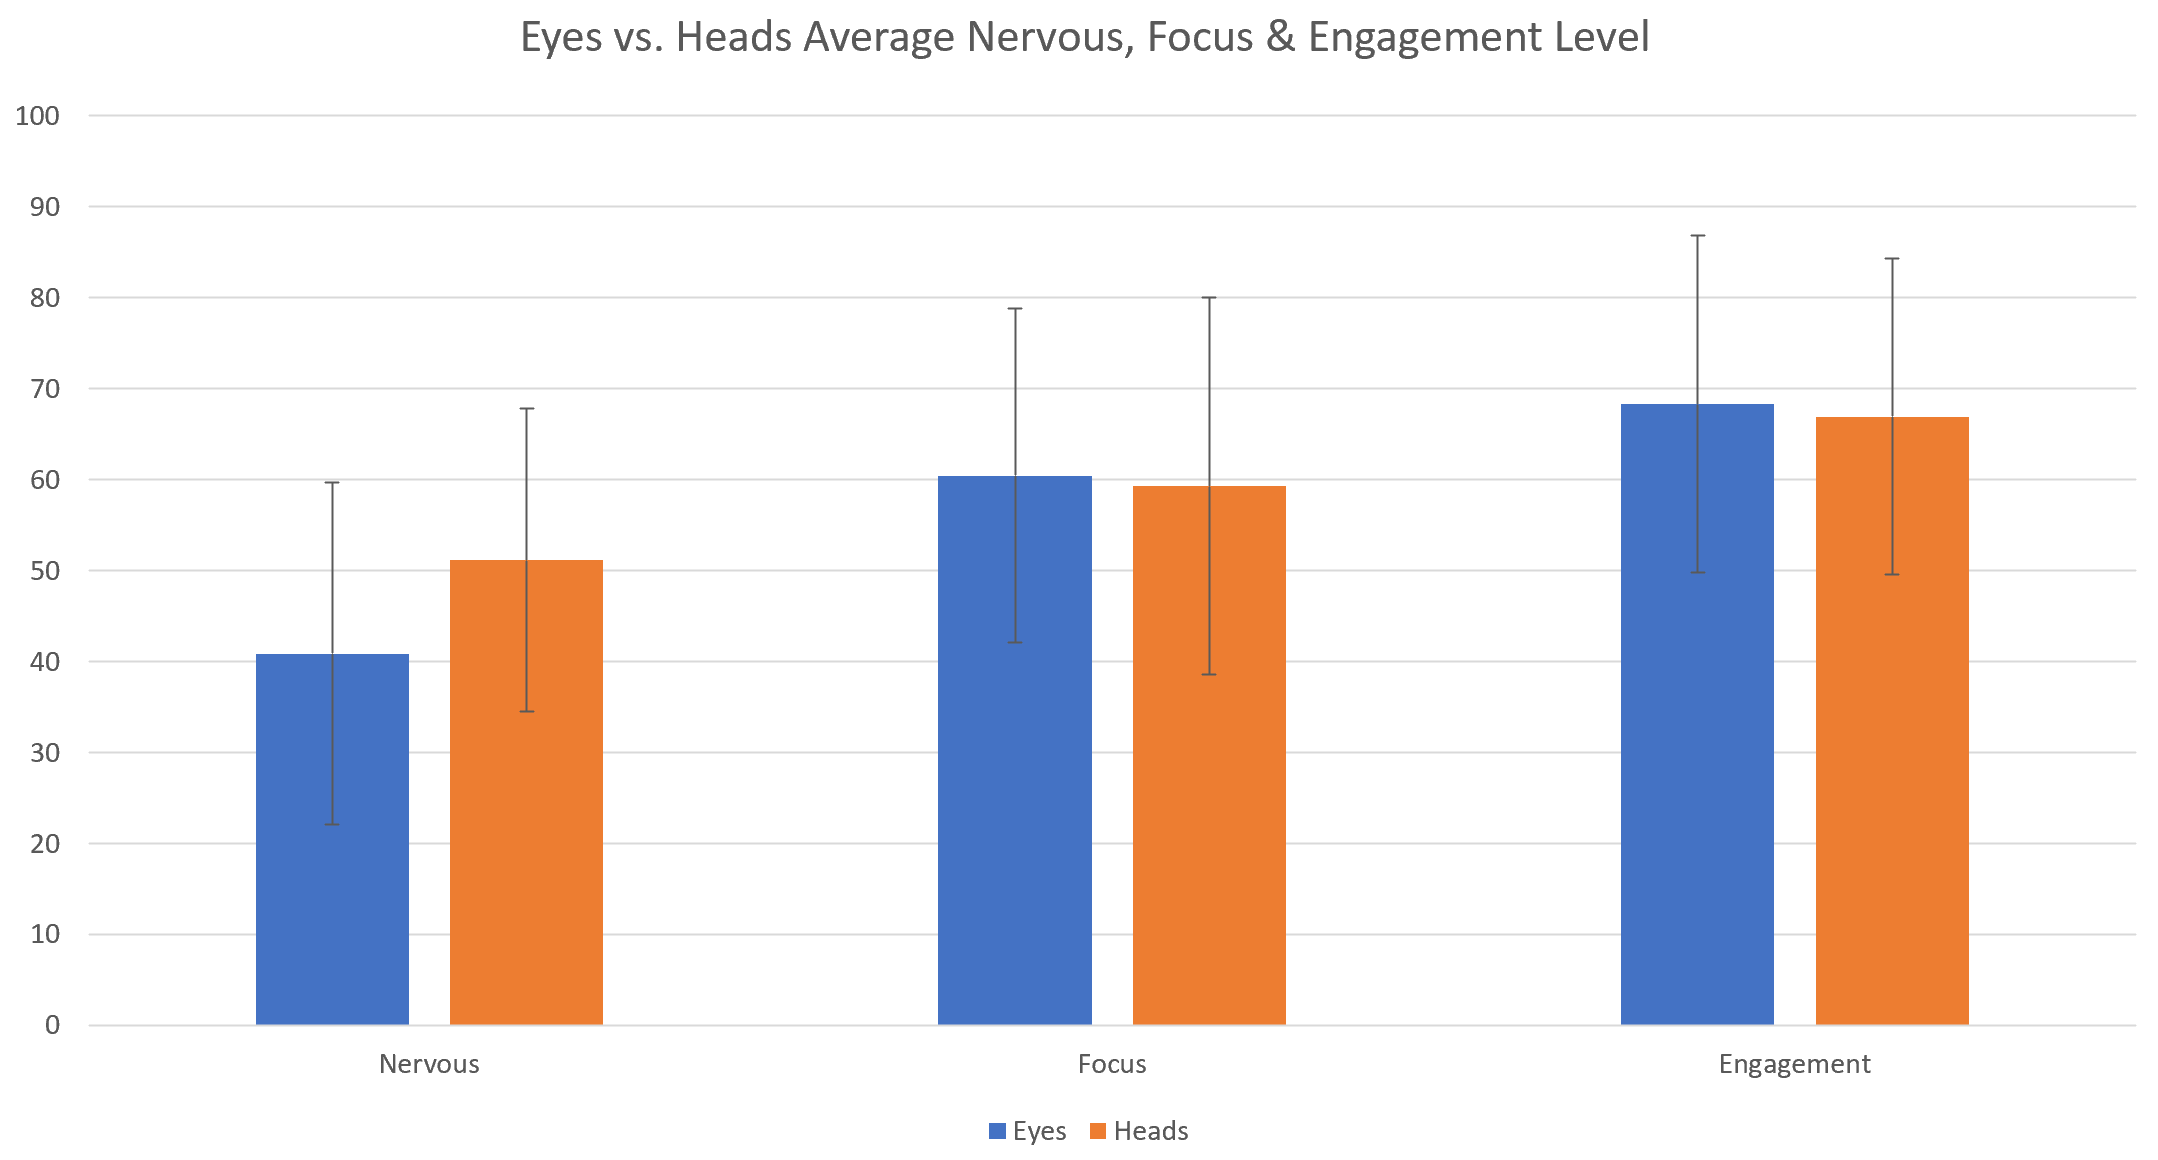
\includegraphics[width=\textwidth]{Result_F3.PNG}
	\caption{Nervousness, focus, and engagement levels reported by the participants as they are asked to speak/present in a room of mock-avatar listeners (E3, H3)}
	\label{fig:e3h3}
\end{figure}

The eye model (E3) average nervous level  is 40.86, and the head model (H3) average nervous level 51.14. This shows that the head model makes participants more nervous than the eye model. The focus level and engagement level for the eye model and the head model does not show significant differences. However, participants reported their focus level and engagement level are enhanced (average focus level is 60.43 for E3, 59.29 for H3; and average engagement level is 68.29 for E3, 66.93 for H3) compared with traditional WVC systems. 


% \textbf{//////////////////////////////////}
% \newline 

The relationship between A,B,C,D were much observed and interpreted clearly (universally) when using heads (H4).
P1, P5, P9, P11, P13 all think compared to the eye model, the head model is much easier to interpret the relationships among other people.
Furthermore, P1 and P5 noted that a few avatars were not participating in the mock-discussion as much.

Unfortunately, while attempting to do quantitative analysis on participant-submitted relationship matrices, we observe that the values in the arrows shown in Figure \ref{fig:relmatrix} were more
closely related to the dynamics in the dialog, rather than eye contact or gaze.

Figure \ref{fig:matrix-mse} shows the mean-squared error (MSE) of the relationship matrix response.
Eventhough users reported having an easier time
seeing using head avatars, they were not any better at correctly perciving the interaction and relationships.
There average increase in misperceptions/errors when switched to heads; and according to user responses,
this could be attributed to head avatars being more distracting.
But it's worth noting that the best-case of MSE decreases when switching from eyes to heads.

Finally, Figure \ref{fig:matrix-attention} shows the magnitude of the user responses between eye avatars and head avatars.
There is a slight increase in percived attention amongst avatars when using heads.
However, this change is very insignificant and could be result of variance/noise.

Generally, the relationship matrix study is not conclusive, and more scenarios and test participants is needed.

\begin{figure}
	\centering
 	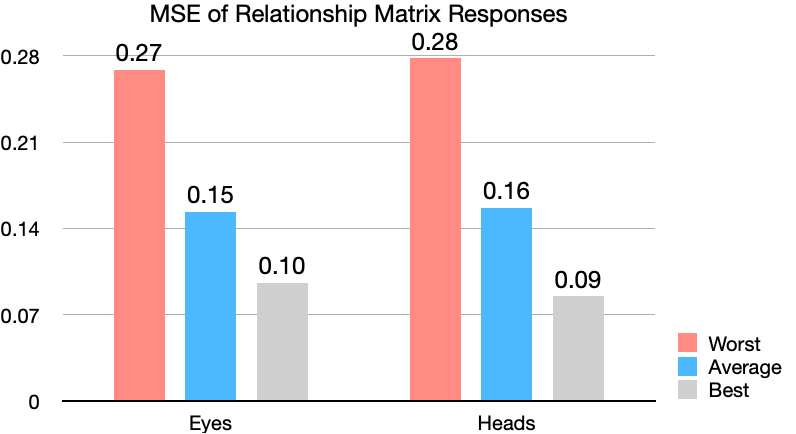
\includegraphics[width=\textwidth]{matrix-mse.png}
	\caption{Mean-squared error of relationship matrix responses (E4, H4)}
	\label{fig:matrix-mse}
\end{figure}

\begin{figure}
	\centering
 	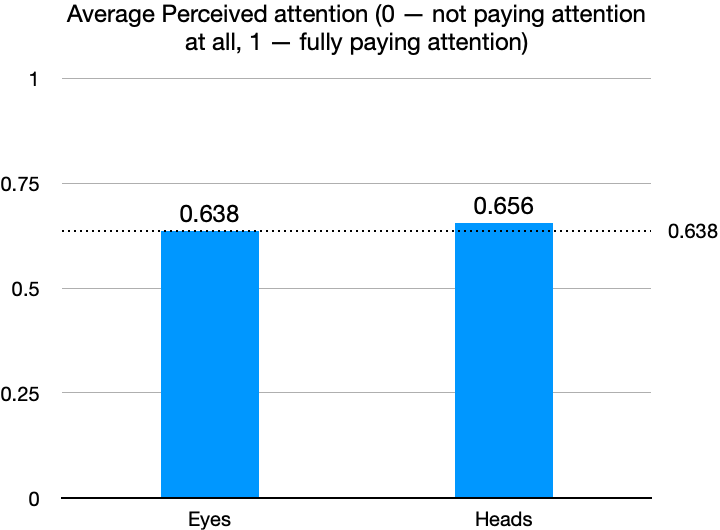
\includegraphics[width=\textwidth]{matrix-amp.png}
	\caption{Normalized mean magnitude of the responses (higher means more percieved attention) (E3, H3)}
	\label{fig:matrix-attention}
\end{figure}




% \begin{figure}
% 	\centering
%  	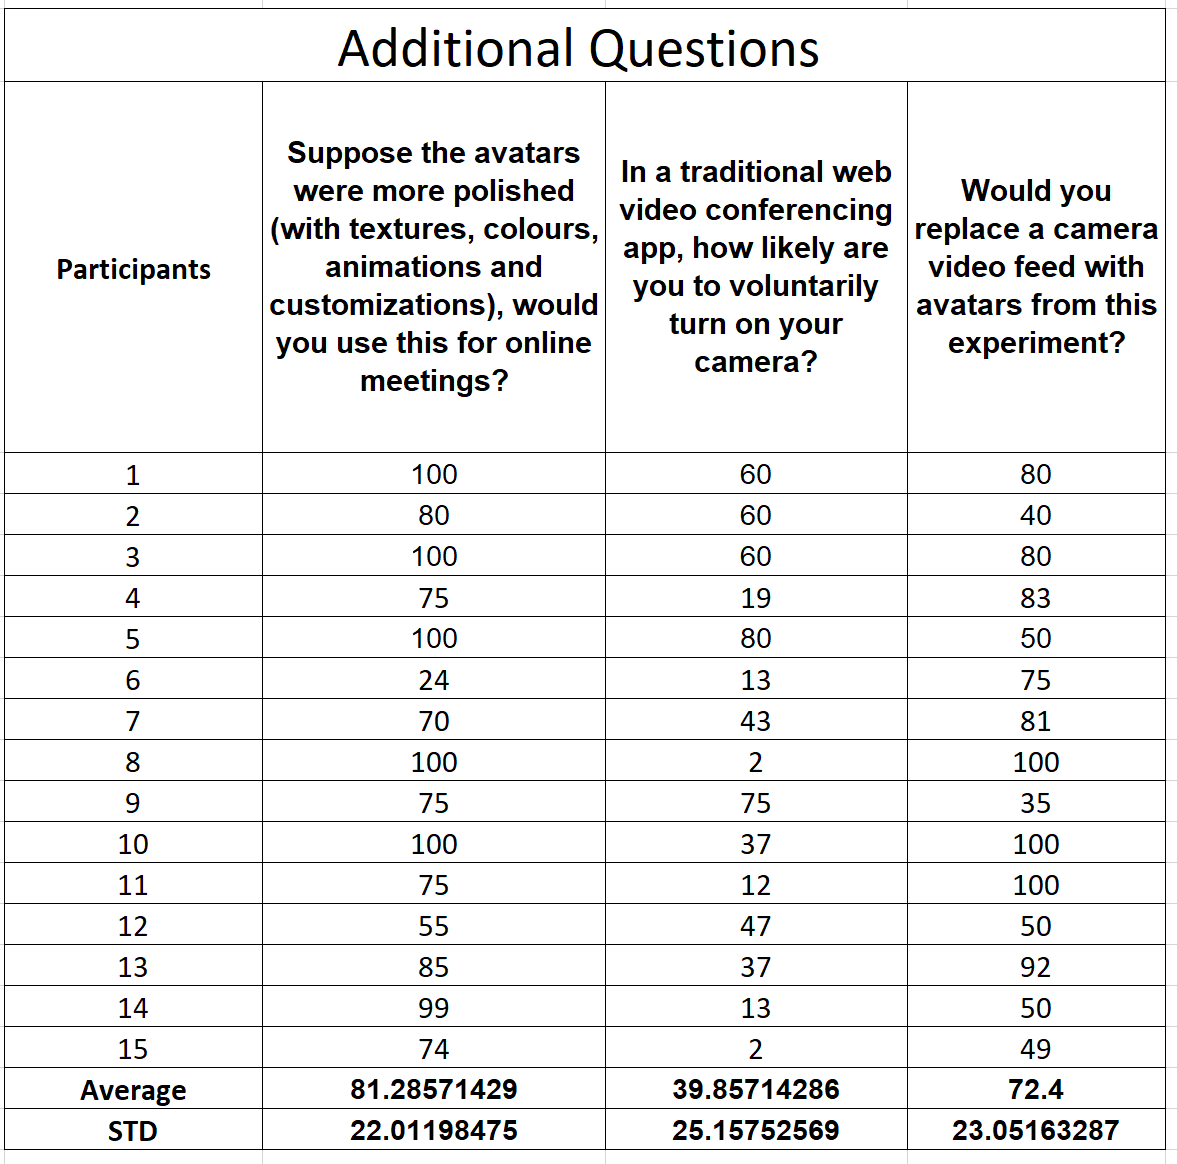
\includegraphics[width=0.45\textwidth]{Result_T1.png}
% 	\caption{The eye model and head model gaze and glimpse times comparison with ground truth}
% 	\label{fig:e1-ga}
% \end{figure}

Participants generally want to use head avatars for online meeting if the avatars were more polished. (Average 81.29 STD 22.01) 
Participants generally would feel comfortable (Average 72.4 STD 23.05) replacing their camera video with the head avatar in certain situations, such as when they don’t want to be distracted by what people are wearing, background, or if themselves don’t want to be seen. 


\section{Discussions}

In general, participants rated the eye model makes them feel less nervous than using traditional WVC systems (average nervous level is 40.86, around 9\% less than neutral). However, comments from participants about nervous level are a bit polarizing. P8 thinks the eye model makes him less nervous since ``\textit{Using cartoon eyes to hide the actual person also makes me less nervous.}" P9 has the opposite opinion about this, ``\textit{Only by showing participants' eyes ... makes me more nervous because you can find out whether people are directly gazing at you anytime.}"
Some participants (P3, P5) also indicated that how nervous they felt depends on how comfortable they are with public speaking. If they’re comfortable talking with a large group of people, neither eyes or heads make a difference in nervous levels. P10 thinks he could not accurately rate his nervous level due to his personal preference of looking away from the screen while talking. It made us to think the possibility of implementing an optional feature to always render the presenter’s view on the audience to help those people who do not have strong public speaking skills to reduce their nervous level. 

Some participants (P3, 5, 9, 10, 15) noted that the head movement in the head model is actually more distracting than the eye model. P10 commented  ``\textit{The movement of the head on the screen may break my train of thought.}" P9 also expressed a similar perspective, ``\textit{Looking at people's heads would make me less focused and nervous because I will pay some attention to them and find out whether they are listening or not.}" Indeed, even when users are giving a talk in real life, they would only perceive the general reactions of the majority of the audiences. They might not notice when only a few audiences start to look around as long as the majority is paying attention. But our system augmented the ``looking around" movement, which made it very obvious when only a few heads start to shift attention despite that the majority are still paying attention. P5 resonated in the same way and felt disappointed when somebody starts to look around.

 

Focus level between eyes and heads are divided: some people (P3, P5) think that the eyes have less focus because it’s hard to tell who is paying attention. On the contrary, P3, 5, 9, 10, 15 think that head is too obvious and the added animation/motion is more distracting. 
P1, 2, 8, 9 commented that head model is more obvious than eye model. 
P3, 5, 9, 10, 15 noted that the head movement is actually more distracting than the eye model.  

Some participants gave comments beyond our questionnaire after they finished the entire experiments. They indicated that in general, they felt more comfortable with the eye model if they are the one talking, but more comfortable with the head model if they are listening. 
They also suggested that for future work, we should also look into combinations of eyes and heads. They also suggested that we could build a model which provides a combination of eyes and heads interchangeably depending on the needs of the users. They could choose to go into head mode when they are listening to a talk and go into eye mode when they are giving a talk.

P7 brought up a point related to privacy, ``\textit{it’s a  pretty interesting app, which helps keep privacy while enabling interaction.}" Privacy is one of the most controversial problems in online meetings during the pandemic period and solutions like virtual background helped to protect the meeting room privacy but not the user's appearance. Using our app, users could choose to not render their camera feed but an avatar head version of themselves. However, in order to achieve this, real time 3D head reconstruction, WVC, and gaze tracking need to be further integrated.


\section{Limitations \& Future Work}

Our project leveraged Unity and Processing to build a proof-of-concept WVC system. We investigated machine-learning-based gaze-tracking technologies and real-time avatar rendering. We also implemented our own WVC system and we successfully integrate it with gaze-tracking technology. But we realized that it is very time consuming to achieving real-time avatar rendering, especially considering this is a course project. We decided to build mock meeting scenes and implemented pre-programmed avatars in Unity to avoid spending time on achieving real-time rendering. The main goal of the paper is to explore the impact and usefulness of eye-contact in WVC system rather than making a working product.

The major limitation is that the avatar may not be as realistic as the human face. So, talking to an animated head with fake eyes may not give the participants the same eye contact experience as in real life. The number of participants in the meeting is another drawback of this prototype; if there are more than 15 participants, their avatars would be arranged into more than one page. While we can overcome the arrangement issue trivially by programming a custom front-end, each participant will have a tiny grid, making the gaze-tracking component a challenge. 

5 participants (P4, P6,  P10, P8, P11) mentioned details on pupils that can be further improved. As P10 described,  ``\textit{typically heads do not move as much during traditional online meeting apps and once someone else is speaking, eyes will shift rather than heads.}" P8 also thinks that our head model does not reflect the real life situation good enough because there are no pupils in the head. P8 said ``\textit{I think it is a good idea to represent people with fake heads, but their eyes did not have a pupil so it was hard for me to tell who is looking at whom based on the eye movement.}" P6 agreed with P10 and mentioned head models without pupils is unnatural for them to look at. Additionally, P4 noted that our eye model is not very realistic since the eyeballs in real life will not be fixed when people are paying attention; people turn their heads and keep blinking their eyes rather than having their eyes fixed. P11 also indicated that ``\textit{The eyes of the avatars could be detailed and optimised for better attention catching for the audiences.}"

After all experiments, we asked participants for their feedback and suggestions for improving our system. Most participants complimented our system and one participant said ``\textit{It's nice enough for me to use it.}" There are two most common suggestions we gathered from the participants. First, improving the rendering quality of the avatars (P4, 7, 8, 9, 10, 11). P4 mentioned \textit{``Obviously, if the avatars are more vivid, and they do represent your eye contact, your direction of looking, maybe even body gesture etc, it could be significantly improving how it is, and avoiding the nervousness and awkwardness with real images." }However, the trade-offs of implementing more realistic avatars need to be considered carefully. P8 thinks the current head model in our system is less realistic, \textit{ ``I think the talking head version is somehow less realistic than the eyes version. Maybe it was because the head is trying to be more realistic, but it is still different from how a real head looks, so it breaks immersion for me."} With more realistic avatars, uncanny valley phenomena might arise. When the head model is closer to the realness but some tiny differences still exist, people tend to feel very comfortable. It also has the risk of breaking the immersion. 

Second, adding more functionalities to the avatar (P2, 4, 10, 12), such as body gesture (P4), head nodding (P2), mouth animation(P10), and customization of avatars (P10) would make our system even better. Two participants (P1, 12) mentioned they’d like to see more features for our system. For example P1 commented ``\textit{give option to switch between 2d and 3d}". P6 thinks our system makes people feel more interactive. They stated that `` \textit{I'd like to see that the avatars could reflect some states of the people who are participating in a virtual conference. This will truly make people feel more interacted.}" 

% - Covid-19 working remotely, so it’s hard to sync up between team members
% - Technical limitations (technical)
% 	- 2D and 3D avatars/views are primitive (barely colours and textures)
% 	- Not customizable, could affect how people feel about usability because it doesn’t convey as much expression as originally intended
% 	- 3D head lack eyes with animation and texture (unfinished due to technical and time constraints) -- also affects how people perceive eye-contact in WVC because it looks creepy (and literally have no eyes).
% 	- Primitive lighting in 3D environment (simple directional light creates uncanny environment)
% - Limitations in running the experiments:
% 	- User testing extremely difficult, despite the prototype framework being cross-platform, exporting/deploying apps required notarization (a security feature that only allows officially signed app to run), so we need last-minute hacks to have the user experiments run
% 	- Small sample size
% - Limitations in collection of data
% 	- Ideally, we want to use some gaze-tracking hardware/software to actually track and log where the users are looking at (as seen in the omitted experiment setup using Tobii), but because none of the user experiments are performed in person, we physically cannot collect those data.
% 	- A workaround is to have the user click/move the mouse to where they’re looking at, but because of aforementioned platform limitations, we can’t do that either
% - Bias of data
% 	- Sample size could be to homogeneous (break down of first-spoken language, ethnicity, geographic location)
% 	- Time of day when running the experiment affects participant’s attention, energy, and mood, and ultimately affect experiment outcomes

% \subsection{Prototype Development}

% - Unified 3D framework/engine
% - Apple Gatekeeper notarization 
% - More sophisticated 3D models and animations
% - Add real-time gaze tracking support
% - More dynamic and fluid 3D environment (since right now all the heads and eyes are locked onto a grid)
% - 
\section{Future Work}

This section talks about the future work

- Testing a combination of eyes and heads
- Testing a large grid of eyes vs. Heads 
- Different combination of styles of eyes and heads

Explore how avatars can move in the space -- what if the avatars can scale based on attention, what if the avatars move back and forth (z direction) based on attention? What you can physically move around in the space

Improvement to the avatar models:

- head nodding
- breathing
- mouth shapes
- hand gestures
- improved randomization
- improved blinking

We would also like to see how this concept can extend to other fields:
- how we can incorporate ML and facial expression recognition technology
- reduce on internet bandwidth for less fortunate participants (lowers data usage)
- 







\section{Conclusion}

% Appendix (uncomment to enable appendix)
% \clearpage
% \appendix
% \section{Appendix name}\label{appendix:sample-appendix}
% Content here

\end{document}
